\section{Realizacja projektu}
Realizacja projektu Meetspace została podzielona na kilka etapów. Pierwszymi z nich było przygotowanie środowiska, zarejestrowanie domeny i zaprojektowanie modelu aplikacji. Następnie rozpoczęły się prace nad poszczególnymi funkcjonalnościami aplikacji, których etapy powstawania zostały udokumentowane w pliku \emph{CHANGELOG.md}


Poniżej zostały opisane wybrane funkcjonalności, działania i zagadnienia z zakresu back-ednu\footnote{działania aplikacji wykonywane po stronie serwera}, front-endu\footnote{działania aplikacji wykonywane po stronie przeglądarki intenetowej} i bezpieczeństwa aplikacji.
  \clearpage
  \subsection{Model bazy danych}
    Do przechowywania danych w aplikacji została wybrana baza SQlite, która w przyszłości zostanie zmieniona na MySQL. Baza zawiera cztery tabele:
    \begin{itemizeReduced}
      \item User - informacje o użytkowniku aplikacji
      \item Event - informacje związane z wydarzeniem
      \item Authentication - informacje pobrane z facebook api
      \item Subscriber - lista osób zapisanych do newslettera
    \end{itemizeReduced}

    \begin{figure}[h]
      \centering
        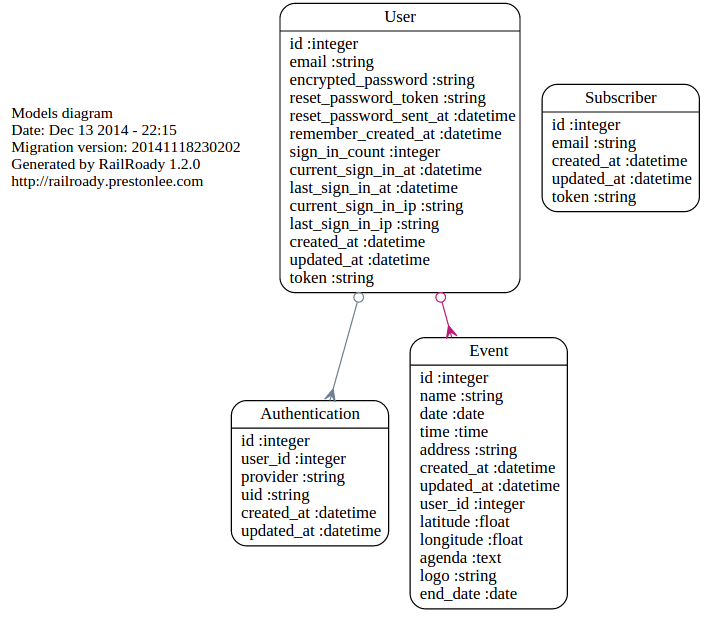
\includegraphics[scale=0.55]{images/dbm.png}
      \caption{Schemat bazy danych aplikacji Meetspace}
    \end{figure}

    Na rysunku nr \ref{fig:dbm} zamieściliśmy schemat bazy zapisany w pliku \texttt{schema.rb}, wygenerowany za pomocą mechanizmu migracji\footnote{Mechanizm wbudowany w Ruby on Rails pozwalający na modyfikowanie bazy danych za pomocą specjalnych plików, tzw. migracji opisujących poszczególne elementy bazy\cite{rails4_way}}.

\begin{code}
  \lstinputlisting[language = Ruby, basicstyle=\ttfamily\scriptsize, showstringspaces=false, breaklines=true, linerange={2-55, 57-57}]{../meetspace/db/schema.rb}
\end{code}


    \subsection{Wyszukiwanie wydarzeń}
    \subsection{Newsletter}
    \subsection{Przykładowe CSS i JS}
    W aplikacji zostały użyte takie technologie jak SASS\footnote{Więcej informacji w rozdziale \ref{other_technology}} i CoffeScript\footnote{Więcej informacji w rozdziale \ref{other_technology}}, które ułatwiły pracę nad wyglądem strony oraz jej funkcjonalnością po stronie przeglądarki internetowej.
    \subsection{Bezpieczeństwo}
      \begin{itemize}
        \item current\_user
        \item boot
        \item autoryzacja api
        \item walidacje
        \item SQL injection
        \item XSS
      \end{itemize}
    \subsection{Przegląd widoków aplikacji}
      \begin{itemize}
        \item responsywnść, czli o gridach
        \item html 5, a co jak nie działą :P?
      \end{itemize}

